多核CPU的出现和快速发展推动了共享内存并行计算平台的接受度。CPU提供了笔记本电脑、台式机和服务器级的并行计算平台,使得它们无处不在。CPU体系结构的最常见形式是缓存相关的非一致性内存访问(cc-NUMA),其特征是访问时间不完全一致。甚至许多小型双插槽CPU系统也有这种内存系统。由于处理器中的核心数量和插槽数量不断增加,这种体系结构已占据主导地位。\par

在cc-NUMA的CPU系统中,每个套接字连接到系统中内存的一个子集。缓存相关的交互将所有的套接字粘在一起,并为开发者提供一致的内存视图。这样的内存系统是可扩展的,因为聚合内存带宽随系统中插槽的数量变化。交互的好处是应用程序可以透明地访问系统中的内存,而不管数据放在哪里。然而,这也是有代价的:内存访问数据和指令的延迟不再一致(例如,固定的访问延迟)。延迟取决于数据存储在系统中的位置。数据来自直接连接到代码运行的套接字的内存。最坏的情况下,数据源于里系统中很远的内存,由于cc-NUMA的CPU系统上插槽之间的数量增加,内存访问成本可能会增加。\par

图16-1是一个具有cc-NUMA内存的通用CPU架构。这种简化的系统架构,包含多插槽系统中的核心和内存组件。本章的其余部分,将用来说明对应代码示例的映射。\par

为了获得最佳性能,需要确保了解特定系统的cc-NUMA配置。例如,Intel最近的服务器使用了网状互连架构,其中核心、缓存和内存控制器组织成行和列。理解处理器与内存的连接性对于实现系统的最佳性能非常重要。\par

\hspace*{\fill} \par %插入空行
图16-1 通用多核CPU系统
\begin{center}
	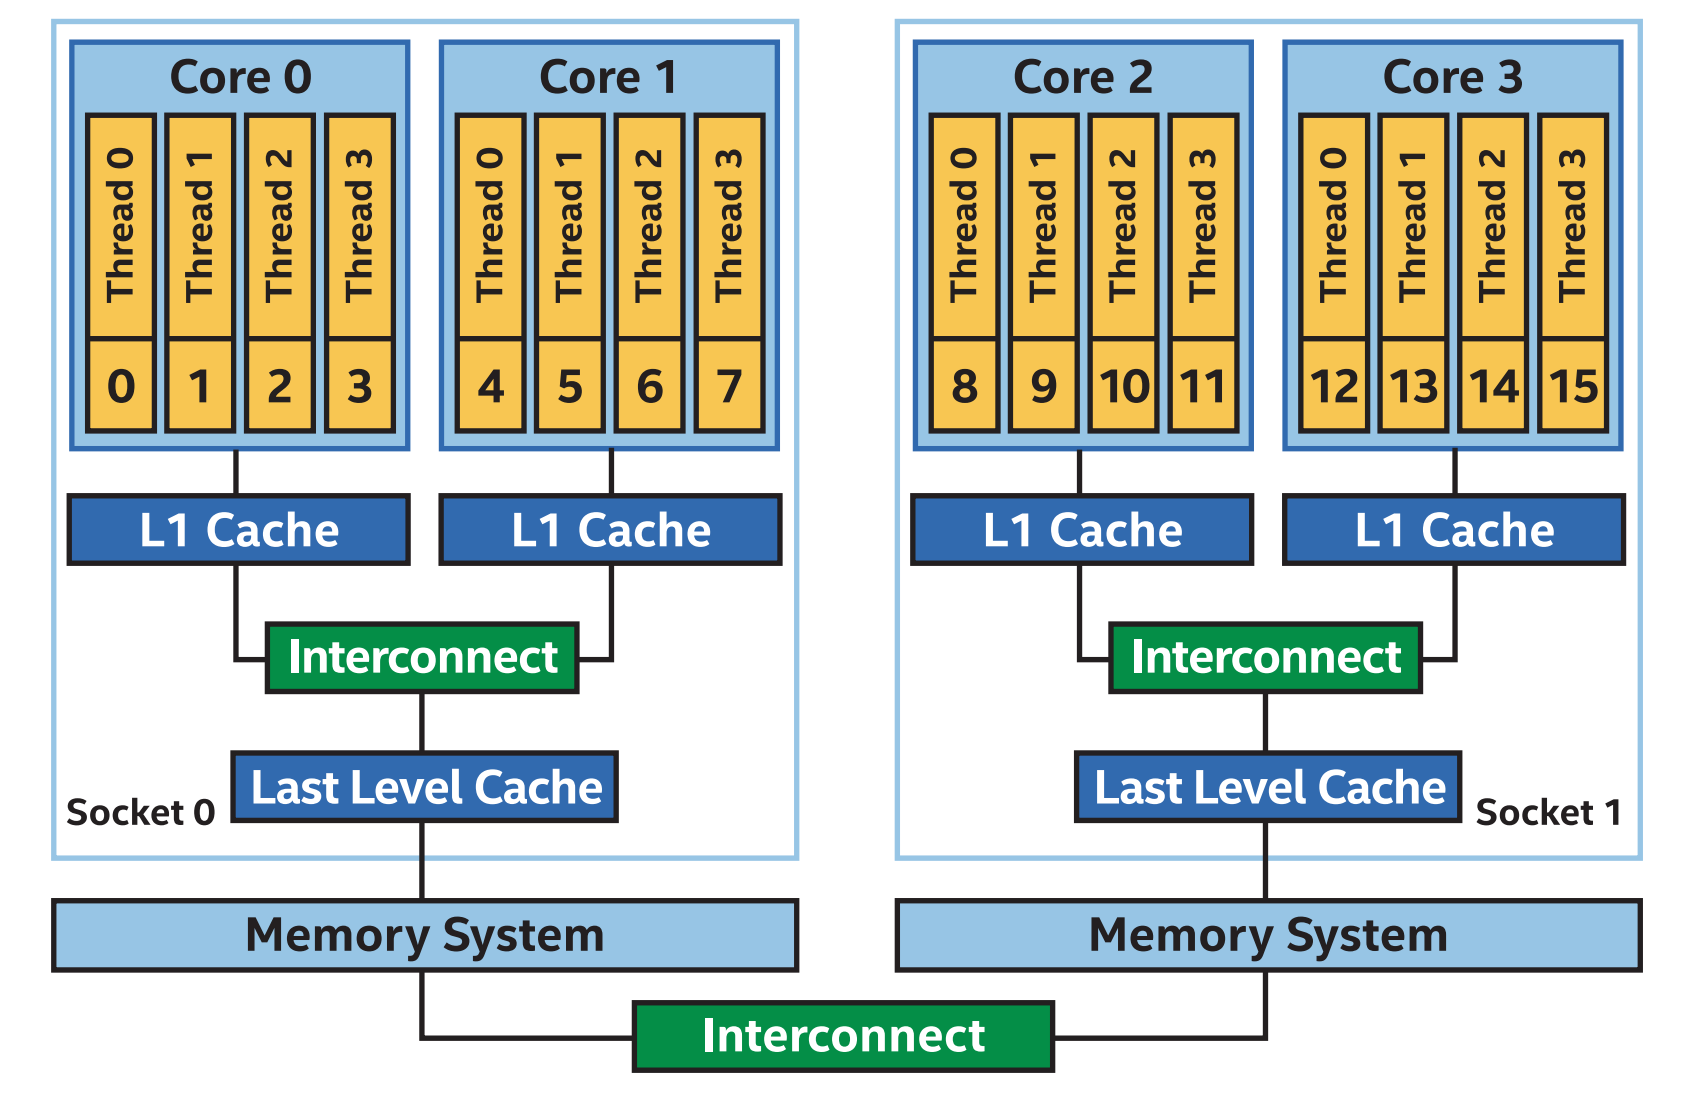
\includegraphics[width=1.0\textwidth]{content/chapter-16/images/2}
\end{center}

图16-1中的系统有两个插槽,每个插槽有两个核,每个核有四个硬件线程。每个核都有自己的一级(L1)缓存。L1缓存连接到共享的最后一级缓存,后者连接到套接字上的内存系统,套接字内的内存访问延迟是一致的。\par

这两个卡槽通过缓存相互连连接起来。内存分布在整个系统中,但是所有内存都可以从系统中的任何地方访问。当不在运行访问内存的代码时,内存读写延迟不一致,这意味着当访问远程数据时,可能会施加不一致的延迟。然而,互连的关键是一致性。不需要担心跨内存系统的数据不一致(这将是一个功能问题),只需要担心访问分布式内存系统的方式对性能的影响。\par

CPU中的硬件线程是执行工具。这些是执行指令流的单元(CPU术语中的线程)。图16-1中的硬件线程从0到15连续编号,这是用于简化本章示例的符号。除特别说明外,本章中有关CPU系统的描述均以图16-1中的cc-NUMA系统为参考。\par




























































